\graphicspath{{07-Absorber/Figures/}}

\section{Liquid-Hydrogen Absorber}
\label{Sect:Absorber}

The accurate characterisation of the properties of the liquid-hydrogen
absorber were a critically important contribution to the study of
ionisation cooling.
The instrumentation used for this purpose and its performance are
presented in this section.

The absorber vessel consisted of a cylindrical aluminium body sealed
with two thin aluminium end windows, as shown in
figure~\ref{Fig:AbsorberVessel:Diag}.
The absorber vessel contained 22\,l of liquid.
The body of the absorber had an inner diameter of 300\,mm and the end
flanges were separated by a distance of 230\,mm.  
The length along the central axis, between the two domes of the thin
aluminium end windows, was 350\,mm~\cite{1748-0221-13-09-T09008}. \\
\begin{figure}
  \begin{center}
    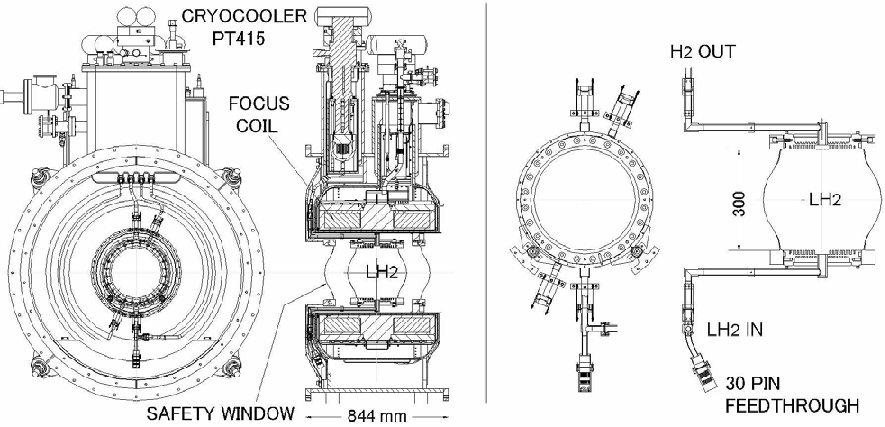
\includegraphics[width=0.75\textwidth]{AFC-drwng.pdf}
  \end{center}
  \caption{
    Left panel: Drawing of the absorber/focus-coil (AFC) module
    showing the principal components.
    Right panel: detail of the liquid-hydrogen absorber vessel~\cite{1748-0221-13-09-T09008}.
  }
  \label{Fig:AbsorberVessel:Diag}
\end{figure}

\noindent\textbf{Variation of the density of liquid-hydrogen due to
    varying temperature and pressure} \\
\noindent
The energy lost by a muon travelling through the liquid-hydrogen
absorber depends on the path length the muon travelled through and on
the density of the liquid-hydrogen. The density of liquid-hydrogen is
a function of temperature and pressure.  
The temperature of the vessel was recorded by eight LakeShore Cernox
1050 SD sensors with a resolution of 0.1\,K. 
Four of the sensors were used solely as temperature sensors, while the
other four were used also as level sensors and exploited to ensure the
liquid hydrogen reached the top of the vessel. 
The sensors were arranged in pairs, with two mechanically clamped at
the top of the vessel, two at a polar angle of ${45}^{\circ}$ to
vertical from the top of the vessel, two at a polar angle of
further rotation of  ${45}^{\circ}$ to the bottom of the vessel, and a
final two at at the bottom of the vessel. 

Cooldown and liquefaction were completed slowly over eight days at a
pressure of 1.15\,Bar after which the vessel's pressure was lowered to
1.085\,Bar~\cite{1748-0221-13-09-T09008}.
The vessel then remained in this steady-state until the
venting process began.
During this process the cryocooler used to liquefy hydrogen was
switched off and heaters were switched on to deliver a nominal power
of 50\,Watt to the absorber vessel
This resulted in an increase in pressure and temperature until the
temperature stabilised at the boiling point.
A rapid increase in temperature was observed once all the
liquid-hydrogen had boiled off. 

The temperature sensors had a typical accuracy of
$\mathrm{\pm}$\,9\,mK and a long-term stability of
$\mathrm{\pm}$\,12\,mK at 20\,K.
The magnetic-field dependent temperature error at 2.5\,T is 0.04\%,
$\Delta$T/T, equivalent to $\mathrm{\pm}$\,8\,mK at
20\,K~\cite{CernoxRTDs}\cite{TemperatureMeasurement}.
These uncertainties were quoted by the manufacturer of the sensors.
Magnetic fields cause a reversible calibration shifts on the temperature
measurements.
To reduce the uncertainty in the liquid-hydrogen density a calibration
procedure was devised that using the boiling point.
A correction to the observed temperature reading was obtained by
applying a cut-off correction, a correction for the effect of the
magnetic field based on the current in the focus coil and its
polarity, a correction for the non-linearity of the sensors, and a 
boiling point scaling factor~\cite{NOTE524}.  
 
The boiling point of hydrogen at 1.085\,Bar is 20.511\,K.
The sensors have a total uncertainty of 17\,mK (9\,mK accuracy, 12\,mK
stability, 8\,mK magnetic).
The deviation from the non-linearity of the sensors adds, on average,
0.03\,K to the uncertainty.
The temperature scaling and magnet-current correction factors also
have an associated uncertainty as they are based on the 0.1\,K
resolution of the sensors.  
For example, a calibrated sensor at boiling temperature and 1.505\,Bar
should read 21.692\,K, but can only read 21.65\,K (21.6\,K cut-off
plus 0.05 cut-off correction) i.e. it is off by 0.042\,K.
The pressure sensors had an uncertainty of $\mathrm{\pm}$\,5\,mBar
which equates to $\mathrm{\pm}$\,0.016\,K during steady state.
The pressure uncertainty ($\mathrm{\pm}$\,5\,mBar) adds another
uncertainty to the temperature calibration constants of
$\mathrm{\pm}$\,0.014\,K.
Collectively, all these uncertainties sum in quadrature to 0.2\,K for
each sensor.
 
In the steady state condition, the liquid-hydrogen was close to the
boiling temperature of liquid parahydrogen~\cite{NOTE524} with a
density of 70.53\,kg/m$^{3}$.
The average temperature of the eight sensors during steady-state was
(20.51\,$\mathrm{\pm}$\,0.07)\,K at 1.085\,Bar
(figure~\ref{Fig:TempCalibrated}) and allows us to determine the
uncertainty in the density as 0.08\,kg/m$^{3}$. \\
\begin{figure}
  \begin{center}
    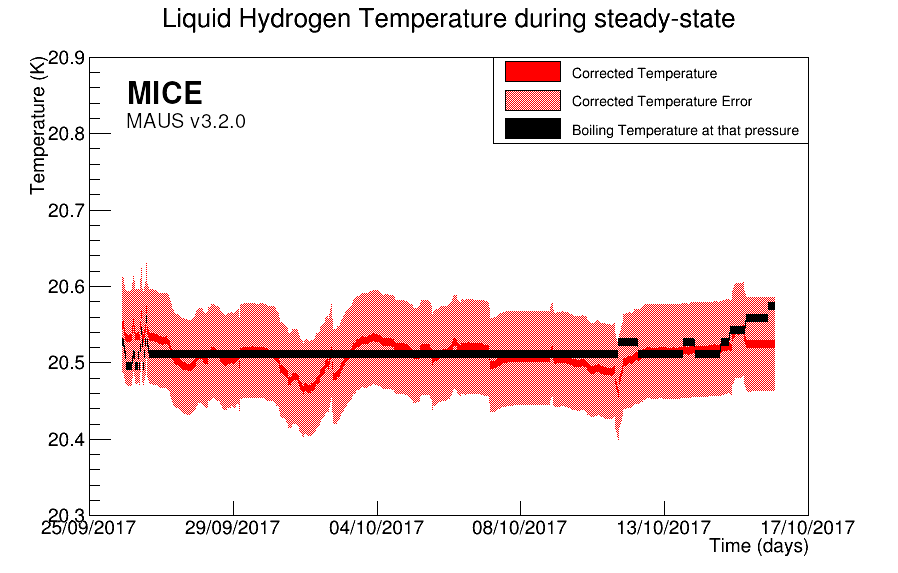
\includegraphics[width=0.80\textwidth]{SteadyState60mK_logo.png}
  \end{center}
  \caption{
    Average LH2 temperature recorded by the sensors during the
    steady-state period.
    After applying all the correction factors the temperature remains
    at or close to the boiling point temperature.
  }
  \label{Fig:TempCalibrated}
\end{figure}
 

\noindent\textbf{Contraction of the absorber vessel due to cooling} \\
\noindent
The absorber was cooled from room temperature to the operating
temperature of the experiment (20.51\,K), which resulted in the
contraction of the vessel.
The linear contraction of Al-6061 as it is cooled from 293\,K is given
by: 
\begin{equation}
  \alpha =-4.1277\times {10}^{-3}\mathrm{T}-3.0389\times {10}^{-6}\mathrm{T}^2+8.7696\times {10}^{-8}\mathrm{T}^3-9.9821\times {10}^{-11}\mathrm{T}^4
\end{equation}
where $T$ is the operating temperature~\cite{Hardin}.
The equation is the result of a fit to data collated by the National
Institute of Standards and Technology (NIST) and has an associated
curve fit error of 4\%. 
At the MICE operating temperature, this corresponds to a linear
contraction of the vessel along each plane of 0.415\%.
As a result the length of the bore contracted by
$(1.45 \pm 0.05)$\,mm.
The vessel was suspended within the warm bore of the focus coil and
was therefore free to contract in each plane without restriction.  \\

\noindent\textbf{Deflection of absorber vessel windows due to internal
  pressure} \\
\noindent
To minimise energy loss and Coulomb scattering by the absorber vessel,
the window thickness was minimised.
It was necessary for the liquid-hydrogen circuit to be pressurised
above atmospheric pressure to prevent air
ingress~\cite{1748-0221-13-09-T09008}\cite{Ishimoto}. 
The vessel was required to withstand a pressure of 1.5\,Bar at which
pressure the the relief valve would operate.

The pressure at which the absorber operated resulted in deflection of
the absorber windows, these deflections were modelled using
ANSYS~\cite{NOTE155}.
The uncertainty in the window deflection derived from the model was
20\%.
The model showed a linear dependence of the window deflection on
pressure up to 2\,Bar when the windows begin to yield.
The pressure sensors were accurate to $\mathrm{\pm}$\,5\,mBar
(0.25\% of 2\,Bar).
At (1085\,$\mathrm{\pm}$\,5)\,mBar, the typical MICE operating
pressure, this corresponded to a deflection of
(0.5374\,$\mathrm{\pm}$\,0.1076)\,mm (model uncertainty)
$\mathrm{\pm}$\,0.0022\,mm (sensor uncertainty) at the centre of the
absorber window. \\

\noindent\textbf{Variation of the absorber vessel window thicknesses} \\
\noindent
On its passage through the absorber a muon would loose energy in the
aluminium of the pair of hydrogen-containment windows, the two
aluminium safety windows, and the liquid-hydrogen itself.
At the centre of the absorber, the total amount of aluminium the muon
beam passes through was (785\,$\mathrm{\pm}$\,13)\,$\mu$m, a variance
of 1.68\%.
However, as the windows were thin, the effects on energy loss were
negligible.
A 200\,MeV/$c$ muon passing along the central axis of an empty
absorber loses 0.345\,MeV, and introduces a 0.006\,MeV uncertainty
on energy loss.  \\

\noindent\textbf{Total systematic uncertainty on energy loss} \\
\noindent
The principal contributions to the systematic uncertainty on energy
loss in the liquid-hydrogen absorber are: the uncertainty in the
contraction of the absorber vessel, the uncertainty in the deflection
of the hydrogen-containment windows due to internal pressure, and the
uncertainty in the variation of the window thickness.
The impact of the contraction of vessel and the deflection of the
windows resulted in a reduction of the length of the of the vessel on
axis of (0.4\,$\mathrm{\pm}$\,0.2)\,mm.
Combined, the change in thickness of the absorber windows on axis
13\,$\mu$m.
The average temperature during the steady state period of the
experiment when the pressure remained constant at
(1085\,$\mathrm{\pm}$\,5)\,mBar is (20.51\,$\mathrm{\pm}$\,0.07)\,K
corresponding to a liquid-hydrogen density of
(70.53\,$\mathrm{\pm}$\,0.08)\,kg/m$^{3}$.

During the MICE data taking, muon beams with nominal momenta of 140,
170, 200 and 240\,MeV/$c$ were used.
The energy loss and its uncertainty were calculated.
The calculation used a central bore length of
(349.6\,$\mathrm{\pm}$\,0.2)\,mm, a total window thickness of
(0.785\,$\mathrm{\pm}$\,0.013)\,mm and a liquid-hydrogen density of
(70.53\,$\mathrm{\pm}$\,0.08)\,kg/m$^{3}$ for a particle travelling
straight through the centre of the absorber. 
For a 140\,MeV/$c$ muon, this corresponds to an energy loss of
(10.88\,$\mathrm{\pm}$\,0.02)\,MeV, while for a 200\,MeV/$c$ muon 
particle this corresponds to an energy loss of
(10.44\,$\mathrm{\pm}$\,0.02)\,MeV.
For a muon travelling along the centre axis of the absorber the
systematic uncertainty in the energy loss is 0.2\%.
